\documentclass[border=2pt]{standalone}
\usepackage[T1]{fontenc}\usepackage{helvet}\renewcommand{\familydefault}{\sfdefault}
\usepackage[helvet]{sfmath}\usepackage{tikz}\usetikzlibrary{positioning,arrows.meta,calc}
\definecolor{dg}{HTML}{1E5A3C}\definecolor{lg}{HTML}{DCE8DF}
\newcommand{\stage}[5]{% name, x, y, number, title; items via #5
 \node[draw=dg,line width=0.8pt,rounded corners=3pt,minimum width=6.2cm,minimum height=3.5cm,anchor=north west,inner sep=0] (#1) at (#2,#3) {};
 \fill[lg,rounded corners=3pt] ($(#1.north west)+(0.4pt,-0.4pt)$) rectangle ($(#1.north east)+(-0.4pt,-0.75cm)$);
 \draw[dg,line width=0.8pt,rounded corners=3pt] (#1.north west) rectangle (#1.south east);
 \node[circle,fill=dg,text=white,font=\bfseries\large,minimum size=0.82cm,inner sep=0] at ($(#1.north west)+(0.38,-0.36)$) {#4};
 \node[anchor=west,font=\bfseries\large,text=dg,inner sep=0pt] at ($(#1.north west)+(0.95,-0.37)$) {#5};}
\newcommand{\items}[2]{\node[anchor=north west,font=\small,text width=5.7cm,align=left] at ($(#1.north west)+(0.15,-0.85)$) {\begin{itemize}\setlength{\itemsep}{0pt}\setlength{\parskip}{0pt}\setlength{\leftmargin}{0.9em}#2\end{itemize}};}
\begin{document}
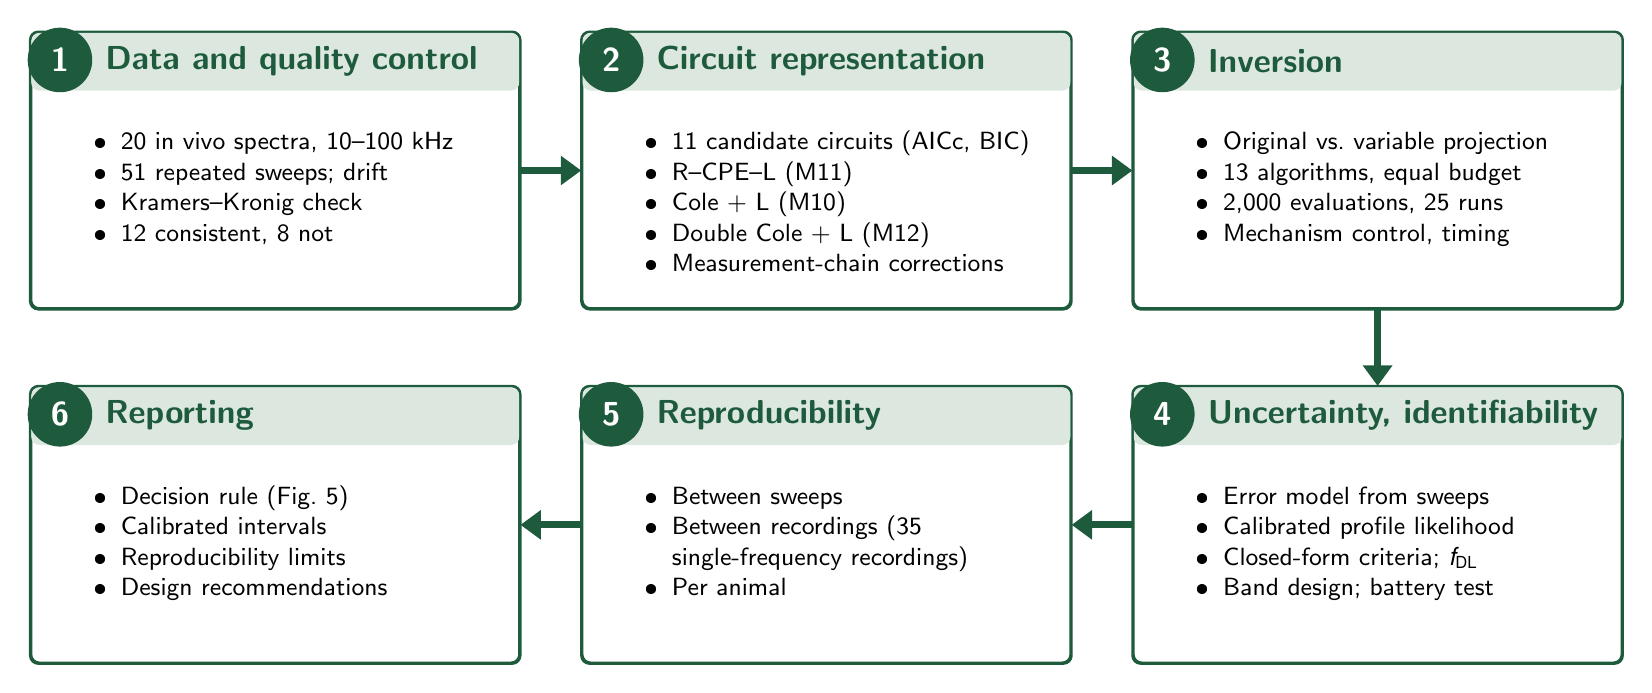
\begin{tikzpicture}[arr/.style={-{Triangle[length=2.6mm,width=3.6mm]},line width=2.6pt,dg}]
\stage{s1}{0}{0}{1}{Data and quality control}
\stage{s2}{7.0}{0}{2}{Circuit representation}
\stage{s3}{14.0}{0}{3}{Inversion}
\stage{s4}{14.0}{-4.5}{4}{Uncertainty, identifiability}
\stage{s5}{7.0}{-4.5}{5}{Reproducibility}
\stage{s6}{0}{-4.5}{6}{Reporting}
\items{s1}{\item 20 in vivo spectra, 10--100 kHz \item 51 repeated sweeps; drift \item Kramers--Kronig check \item 12 consistent, 8 not}
\items{s2}{\item 11 candidate circuits (AICc, BIC) \item R--CPE--L (M11) \item Cole + L (M10) \item Double Cole + L (M12) \item Measurement-chain corrections}
\items{s3}{\item Original vs.\ variable projection \item 13 algorithms, equal budget \item 2,000 evaluations, 25 runs \item Mechanism control, timing}
\items{s4}{\item Error model from sweeps \item Calibrated profile likelihood \item Closed-form criteria; $f_{\mathrm{DL}}$ \item Band design; battery test}
\items{s5}{\item Between sweeps \item Between recordings (35 single-frequency recordings) \item Per animal}
\items{s6}{\item Decision rule (Fig.~5) \item Calibrated intervals \item Reproducibility limits \item Design recommendations}
\draw[arr] (s1.east) -- (s2.west); \draw[arr] (s2.east) -- (s3.west);
\draw[arr] (s3.south) -- (s4.north); \draw[arr] (s4.west) -- (s5.east); \draw[arr] (s5.west) -- (s6.east);
\end{tikzpicture}
\end{document}
